
%----------------------------------------------------------------------------------------
%	CHAPTER 2
%----------------------------------------------------------------------------------------
\chapterimage{chapter_head_2.pdf} % Chapter heading image

\chapter{\textcolor{blue}{ \Bodycontrol}}



%%%%%%%%%%%%%%%%%%%%%%%%%%%%%%%%%%%%%%%%%%%%%%%%%%%%%%%%%%%%%%%%%%%%%%%%%%%%%%%%
%%%%%%%%%%%%%%%%%%%%%%%%%%%%%%%%%%%%%%%%%%%%%%%%%%%%%%%%%%%%%%%%%%%%%%%%%%%%%%%%
\section{ Treino de ombros e quadril no plano frontal}

Figura \ref{fig:pessoalombroquadril1}.

\begin{figure}[!h]
  \centering
    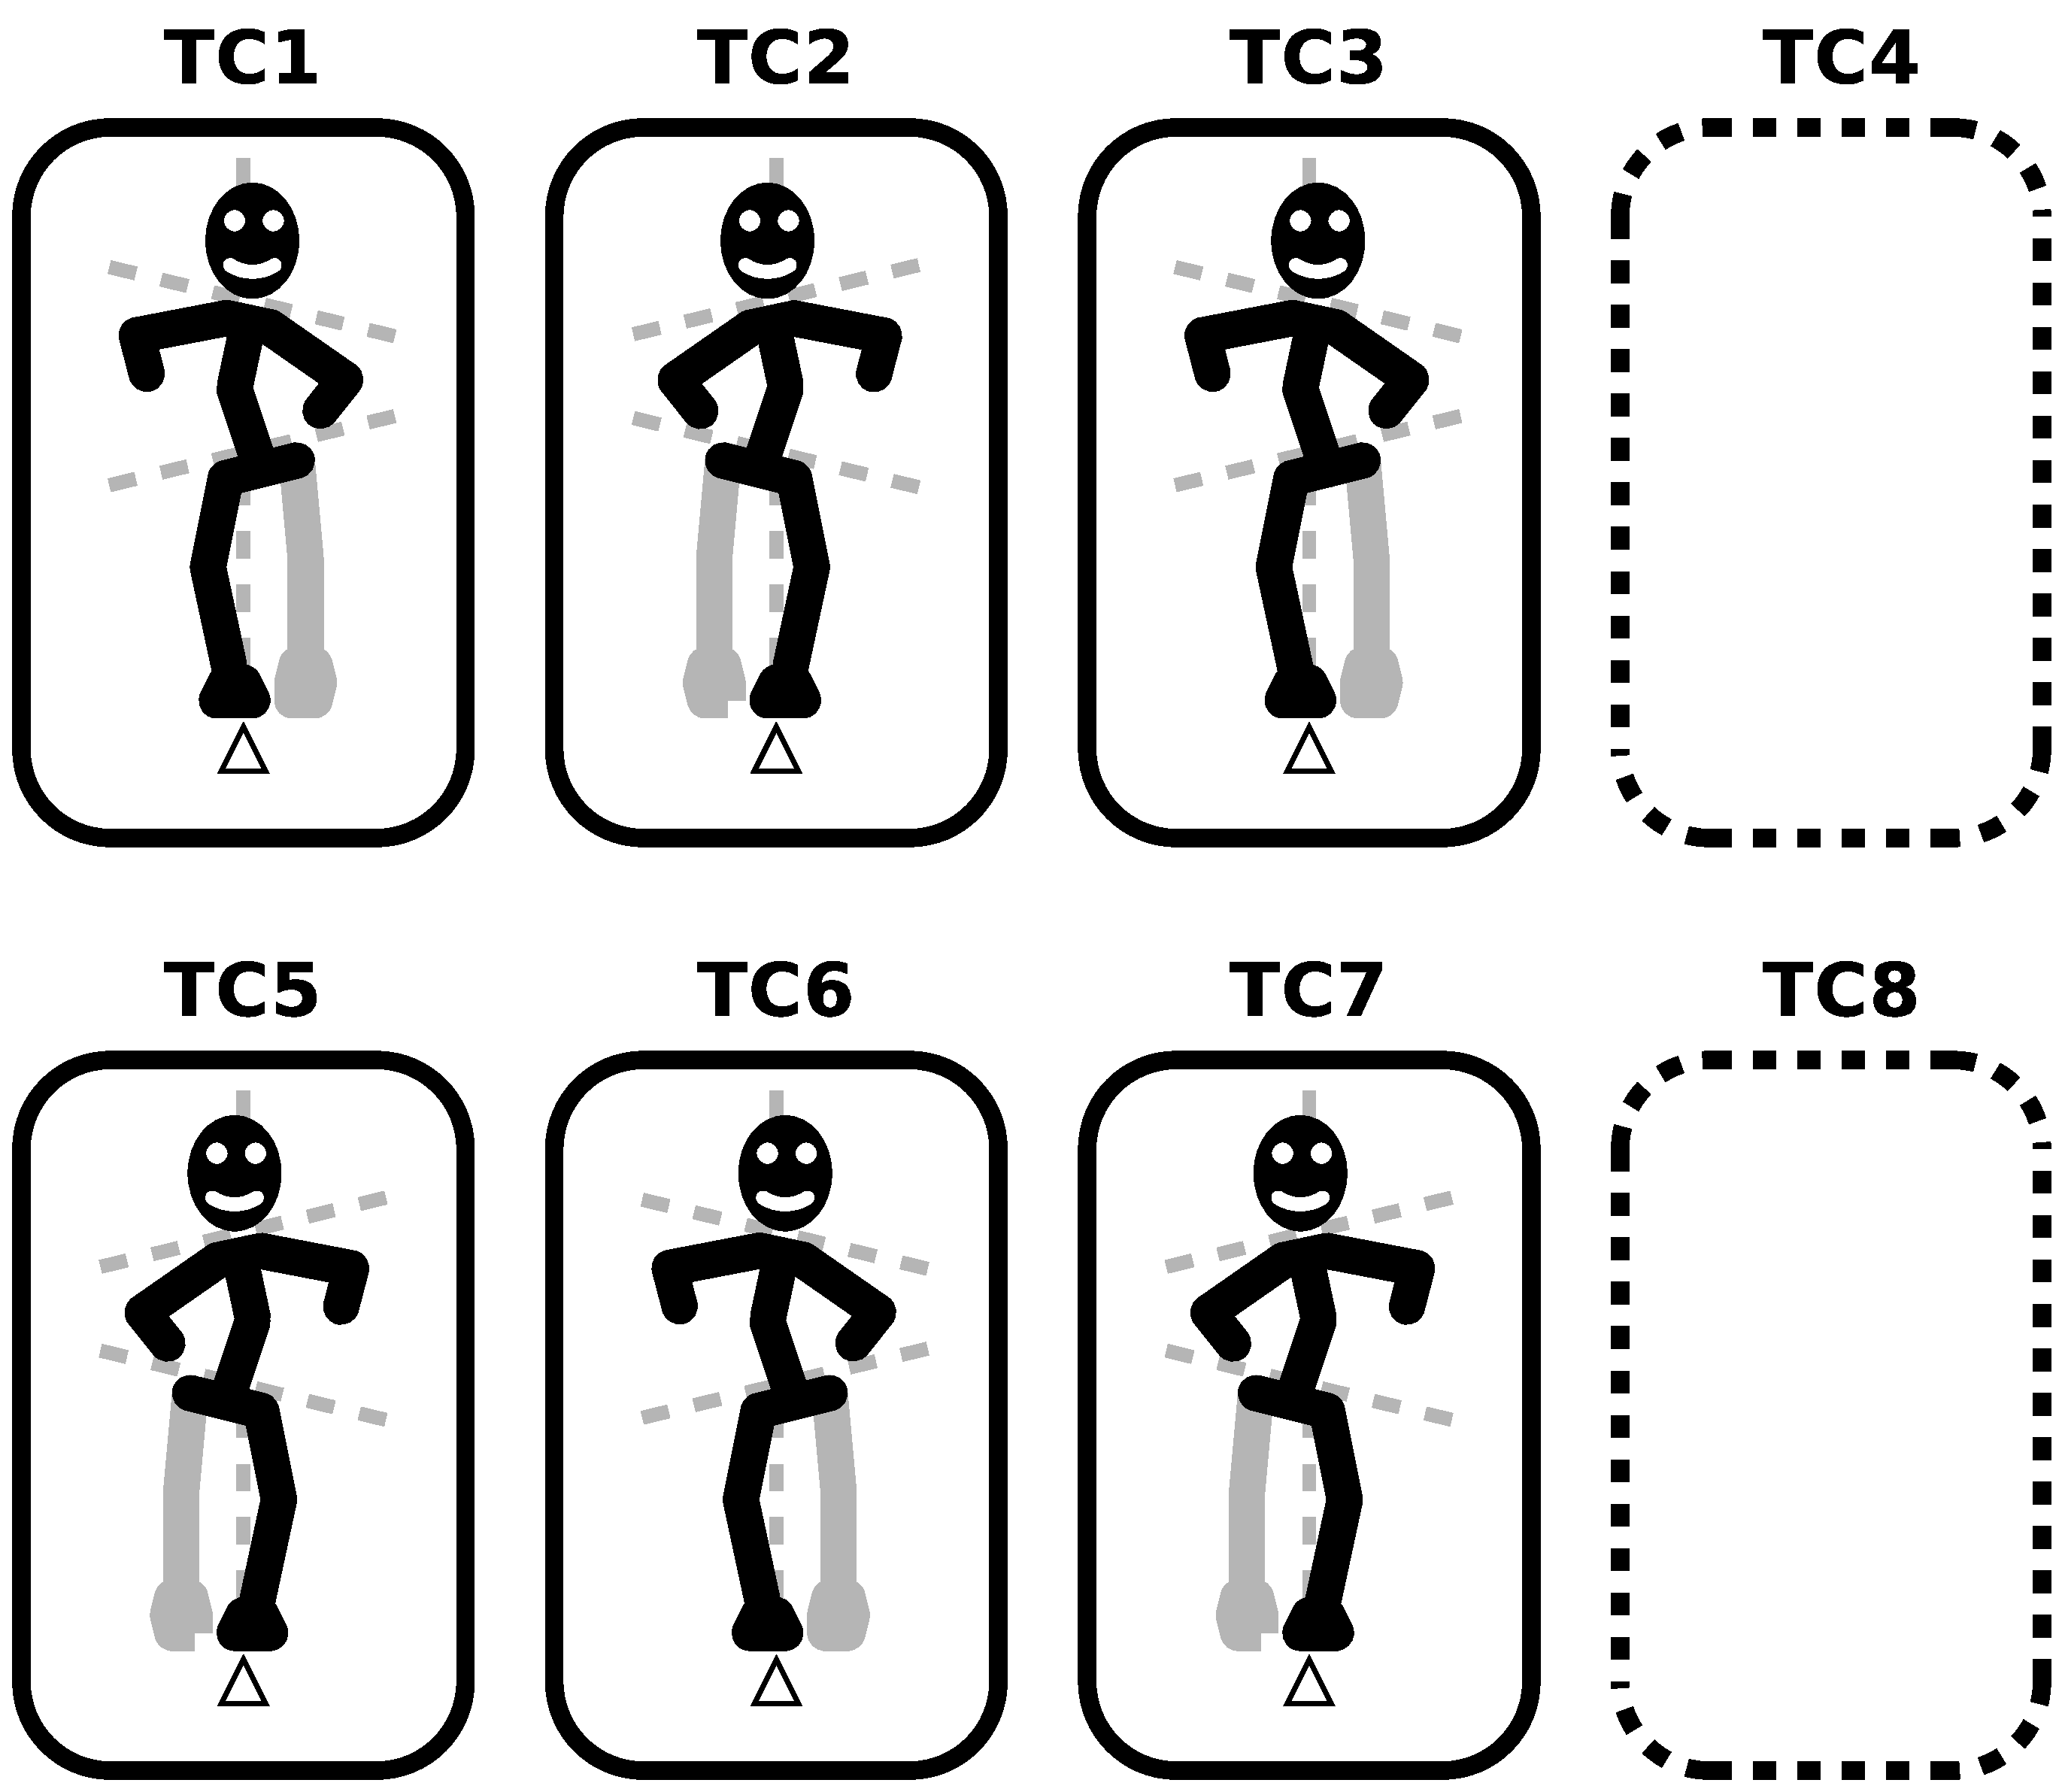
\includegraphics[width=\bodyboxsize]{chapters/cap-body-control/postura-ombro1.eps}
\caption{Diagrama de tempos coreográficos para o treino ombros e quadril, $T=2~TC$.}
\label{fig:pessoalombroquadril1}
\end{figure}

\section{\textcolor{red}{  Treino de ombros no plano frontal}}

\section{\textcolor{red}{  Treino do quadril no plano frontal}}


